\section{Graphic Adapters}
\[ \text{Graphic Adapters Overview} =
\begin{cases}
	Vector \\
	Raster \\
	Accelerated
\end{cases}
\]

\subsection{Vector Graphic Adapters}
This type of adapters are old-fashioned and not used any more. The technology used
is similar to the one in oscilloscopes : a moving , turned on/off \textbf{beam} in a CRT used to draw objects on a screen.\\
Used mainly in '70s in high-end visualisation tools , later in arcade gaming machines ( ex: Atari Battlezone ) and even used in the Vectrex , a home entrainment system.\\
Graphics are drawn as a \textbf{set of commands} sent from software to hardware (adapter). The commands are used to generate \textbf{3 analog} signals that control horizontal \& vertical positions and the beam intensity.
\begin{figure}[!h]
\begin{minipage}{.5\textwidth}
 \centering
  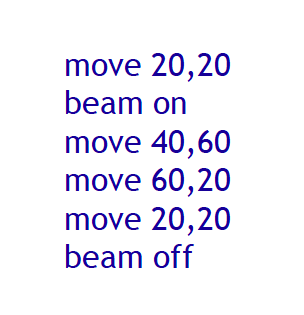
\includegraphics[width=.6\linewidth]{cmd}
\end{minipage}%
	\begin{minipage}{.5\textwidth}
  \centering
  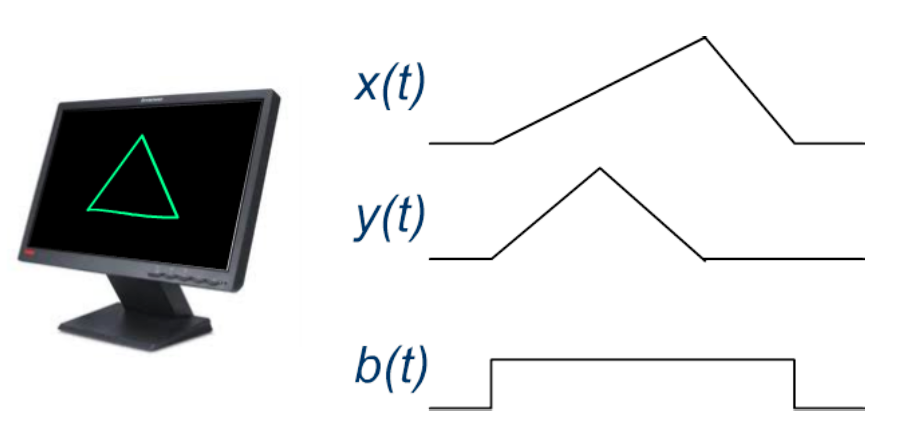
\includegraphics[width=.9\linewidth]{vector}
\end{minipage}%
\end{figure}

\subsection{Raster Graphic Adapters}
Raster graphic adapters divide the screen into a \textbf{matrix} of individually assignable elements called \textbf{pixels} which are assigned \textbf{colors.} If the color comes from a spatial sampling of an image the adapter can reproduce it on the monitor.\\
Raster adapters have a special memory called Video Memory (\textbf{VRAM}) made of cells that contain information about the color of each pixel on the screen. A component on the video card ( RAMDAC for analog displays ) converts the information to the signal required to transfer the image to the monitor.\\
Images on the screen can be written by setting specific values in the VRAM ( \texttt{writeScreen()} function).
\begin{figure}[!h]
 \centering
  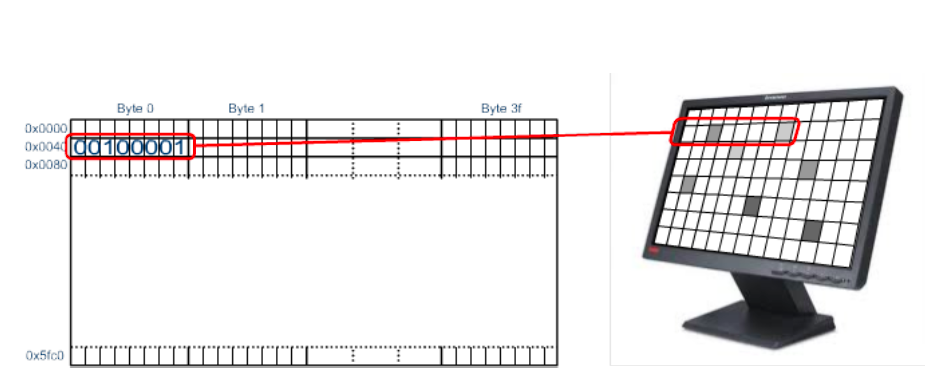
\includegraphics[width=.7\linewidth]{raster}
\end{figure}
Still in used but slowly dismissed due to reduction of hardware costs of better technologies. Initially the memory was just enough to store a single screenshot.\\

\subsection{Accelerated Graphic Adapters}
Are a special kind of raster graphic adapters that have \textbf{much more memory} than the one required to store a single screenshot. Instead of writing \textbf{directly on the screen buffer } ,images are stored in different areas of the VRAM.\\
Commands that can be interpreted by the adapter include :
\begin{itemize}
\item Draw points,lines and other figs
\item Write text
\item Transfer raster images from VRAM to screen buffer
\item 3D projections
\item Deform + effects on images
\end{itemize} 
Used today , these adapters can perform complex tasks ( multi - display screening, stereoscopic images ..)

\subsection{Color vision}
How is color on-screen encoded in bits? Commonly a system called \textbf{RGB} is used.
In the following sections we'll find why.

\subsubsection{Human Vision}
The color of the light is determined by the \textbf{wavelength} of the photons that transmit it. Visible light ranges from 400-700 nm wavelength.\\
Depending on the \textbf{light source} , lots of photons of \textbf{different wavelengths} are emitted. The photons then interact with the environment where objects, depending on their composition , \textbf{reflect or absorb} the various wavelengths at different intensities. The reflected photons are then focused on the retina where \textbf{rods} (sensible to light intensity) and \textbf{cones} (sensible to light color) transmit information to the brain through \textbf{nerves}.\\
There are 3 types of cones $ \rho , \beta ,\gamma$ each sensible to a different portion of light spectrum.\\
By combing the stimuli of different cones the brain allows the vision of a given color.
\begin{figure}[!h]
 \centering
  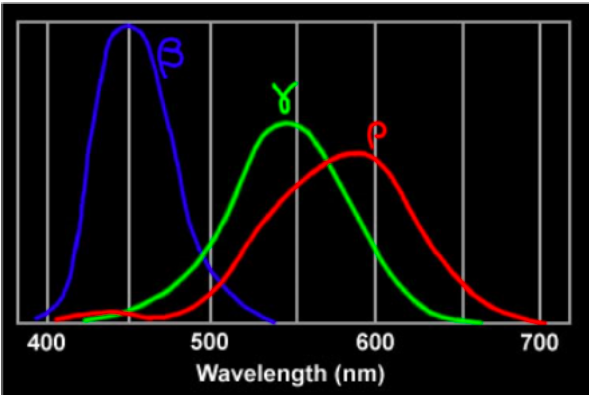
\includegraphics[width=.5\linewidth]{cones}
\end{figure}
\newpage
\subsubsection{Color reproduction}
Color reproduction uses the inverse procedure of the human vision : \\
it associates a different \textbf{emitter} for each color the human cones can capture.
Since the main wavelengths perceived by the cones are \textbf{red, green \& blu} , different hues are constructed by mixing light of these three.\\
Mixing two of three primary colors \textbf{cyan, magenta and yellow} are obtained. Mixing the three in different proportions \textbf{all} possible hues can be obtained.
\begin{figure}[!h]
 \centering
  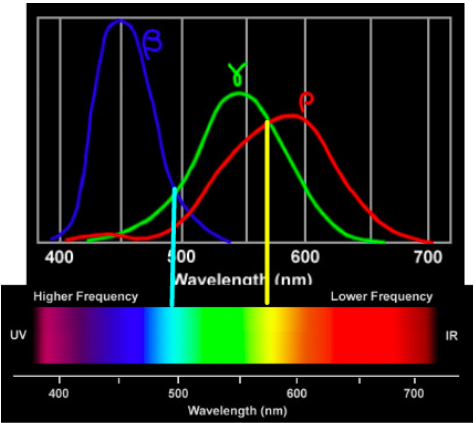
\includegraphics[width=.5\linewidth]{cyanyellow}
\end{figure}
\begin{description}
\item[Color range]\hfill\\
The \textbf{spectrum} that a monitor can produce is just a small portion of the entire spectrum the eye can see (grey area).\\
Color range of a monitor corresponds to a cube where the three colors are placed on the 3 axis.
\item[Color synthesis]\hfill\\
The levels of red green and blue are translated into three \textbf{electrical signals} whose intensity controls the light emitted by the screen for each of the primary colors.\\ \newpage
As the system is digital \textbf{DACs} are used to \textbf{quantize} the signals.
Quantisation further \textbf{reduces} the number of visible colors : quantisation levels 	are usually $ 2^{d/3}$ with \textbf{d} being the number of bits per pixel

\begin{figure}[!h]
\begin{minipage}{.5\textwidth}
 \centering
  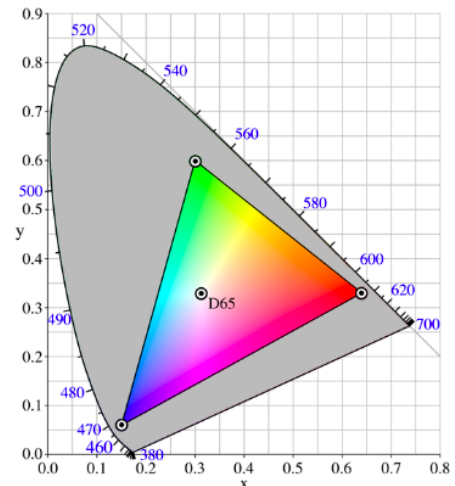
\includegraphics[width=.5\linewidth]{range}
\end{minipage}%
	\begin{minipage}{.5\textwidth}
  \centering
  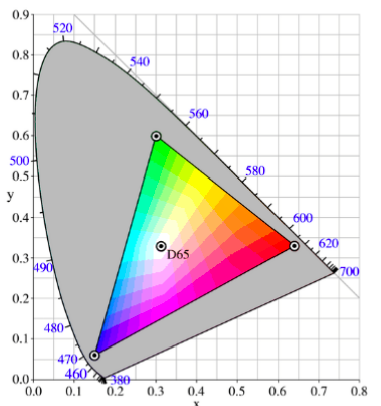
\includegraphics[width=.5\linewidth]{q_range}
\end{minipage}%
\end{figure}
\end{description}

\subsection{Image Resolution}
The resolution of an image defines the \textbf{density of pixels} that compose it.
When dealing with \textbf{raster graphics on screen} the density is relative to the \textbf{monitor size} : the resolution defines thus the number of pixels displayed on the screen on the horizontal (\textbf{width} ) and vertical (\textbf{height}\\
Pixels are not always \textbf{square shaped} so the horizontal resolution $ \neq$ vertical resolution.
\begin{description}
\item[Memory of Images]\hfill\\
Raster images require lots of memory : FullHD up to 6MB $$ \text{Memory} = w * h * d_ {bits} $$
A first way to reduce image size was to reduce the \textbf{colors} using a \textbf{color palette} : a predefined set of colors that contains a \textbf{limited} number of entries.\\
The palette is encoded as an array of \textbf{RGB values}	that are used to define the possible colors that can be used in an image. \\
If the \textbf{color depth d} (number of bits per pixel) is $ \leq 8 $ a color palette is used ( the palette contains $ 2^d$ colors).\\
If a user defined palette is used, the size of the palette must be added to the image size. With p = bits to encode a palette entry $$ \text{Memory} = w * h * d + p * 2_{bits}^d$$
\end{description}
	






